\documentclass[letterpaper, 10 pt, conference]{ieeeconf}


\usepackage[colorlinks=true, urlcolor=blue, pdfborder={0 0 0}]{hyperref}
\usepackage{geometry}
\usepackage{overpic}
\graphicspath{{./pictures/pdf/},{./pictures/ps/},{./pictures/png/},{./pictures/jpg/}}
\begin{document}
\author{Professor Aaron T. Becker}
\title{How to join the Robotic Swarm Control Lab}
\maketitle

\begin{abstract}
The Robotic Swarm Control Lab (RSCL) exists to
 (1) understand, quantify, and implement the best methods for controlling huge numbers of robots, 
 (2)  implement robotic solutions to medical problems, 
 (3)  train confident, productive, ethical engineers to perform impactful research.

This document explains how to earn lab access and the software suite we use.
\end{abstract}

\section{Preliminaries}

We are glad you are interested in the lab!  

\begin{figure}[h]
\begin{center}
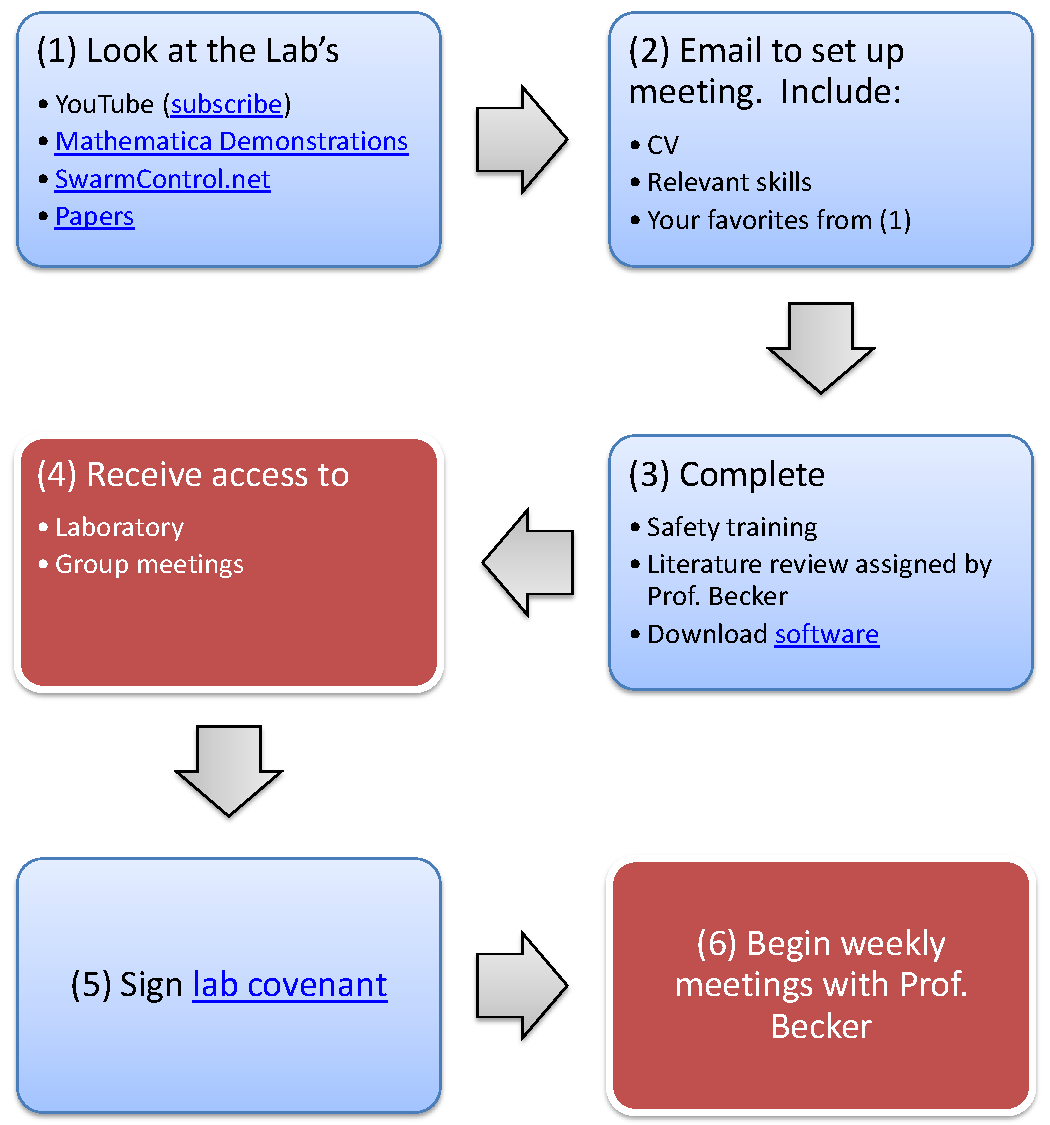
\includegraphics[width=\columnwidth]{JoiningLabFlowChart.pdf}
\caption{Some description of figure.  All plots must have labeled axes with units in parenthesis, for instance:  Robot diameter ($\mu$m)}
\end{center}
\end{figure}


\subsection{Learn about our lab}

\begin{enumerate}
\item Browse through 
 our YouTube channel \href{www.youtube.com/aabecker5/}{youtube.com/aabecker5/}, 	\href{http://demonstrations.wolfram.com/author.html?author=Aaron+Becker}{Mathematica Demonstrations}
Gamification research: \href{www.SwarmControl.net}{SwarmControl.net}, 
and papers: \href{scholar.google.com/citations?user=6kGt1DEAAAAJ}{scholar.google.com/citations?user=6kGt1DEAAAAJ}
o	Decide: 
1.	Do any of these seem interesting to you? 
2.	If so, do you have any tools or techniques that could be applied to these?  
3.	Could you optimize something?
o	Do you already have a project?  
1.	If so, can you show how it aligns with my lab's goals or interests?
2.	Email a one-page document to Prof. Becker explaining 
o	Your potential project, 
o	Why you want to attack this problem
o	Any skills you bring to the project
o	Funding requirements.  Funding MS students is very difficult, funding PhD students is difficult, but there are some opportunities every semester either through my grants or by applying to external sources.
3.	Request a meeting with Prof. Becker, or visit during office hours (at least 12 hours after emailing description)
\end{enumerate}


\subsection{Software}
The following instructions are aimed toward users with Windows operating system. If you use Linux, we will assume you are competent to find your own software.

Our papers are produced in \href{http://en.wikipedia.org/wiki/LaTeX}{\LaTeX}, a document markup language. \LaTeX is widely used for the communication and publication of scientific documents in many fields.

First, download and run the Basic MiKTeX installer to setup a basic TeX/LaTeX system on your computer \url{http://miktex.org/download}

Second, install Texmaker, a front end for \LaTeX \url{http://www.xm1math.net/texmaker/download.html}

Third, install github. We submit our code and written documents through github, which serves as a distributed backup. 
\url{https://github.com/}
https://github.com/aabecker





 
\section{Earning Lab Access}
Every potential lab member must complete a literature review and lab safety training before being issued access to the robotics lab.

\subsection{The literature review}
Master and PhD scholars primarily share their research through scholarly writing in academic journals and conferences. Members of the RSCL must have one conference paper to be eligible for a Master's degree. Every paper begins with an outline of the problem, followed by an overview of the current solutions in this area this is called the \emph{literature review}. To join the lab everyone (undergraduates to professors) must complete the following literature review.

On a topic selected by Prof. Becker, select no less than eight references from the proceedings of ICRA, IROS, or RSS \footnote{Some conferences are better than others, and some journals are better than others. ICRA, IROS, and RSS are the flagship conferences in robotics.  ICRA and IROS have $\approx$1,000 papers each year, RSS is more elite with $\approx50$ papers.} Go back no more than five years.  Older papers have usually been superseded by new algorithms or technology.

The goal is a concise, high-level research summary.  For each paper, write only one paragraph.  There should be less than three papers per column.

\begin{itemize}
\item Goal of their research 
\item Assumptions (centralized control vs decentralized, perfect sensors vs partial state feedback, in simulation or in experiments, etc.)
\item Limitations (what did they actually do?)
\end{itemize}

These summaries should be concise: no more than 3 papers per column.


\subsection{Lab Safety training}

The class \textbf{EH06: General Laboratory Safety and Hazardous Materials Orientation} is mandatory for all lab members. This class can be signed up for online. It is more fun to complete with a friend.

\begin{itemize} 
\scriptsize
\item \url{http://www.uh.edu/ehls/training/}
\item \url{http://www.uh.edu/ehls/training/eh06/}
 \end{itemize}

 
 This class includes toxicology, recognition of hazards, personal protective equipment, understanding MSDS's, proper storage of chemicals, proper disposal of chemicals, fire safety and general safety rules


\section{Conclusion}

To subscribe or unsubscribe via the World Wide Web, visit
        http://duerer.usc.edu/mailman/listinfo.cgi/robotics-worldwide

 
 \end{document}